% Evaluation

\section{Evaluation}
\label{sec:evaluation}

We evaluate \textsc{WasmSentinel} along four dimensions:
(1) detection accuracy on standard benchmarks,
(2) inference latency and throughput,
(3) comparison with state-of-the-art systems,
and (4) impact of architectural choices.

\subsection{Experimental Setup}

\textbf{Hardware.}
Experiments run on a server with:
Intel Xeon E5-2680 v4 (14 cores @ 2.4GHz),
64GB DDR4 RAM,
Ubuntu 22.04 with Linux kernel 6.1.

\textbf{Dataset.}
We use the ADFA-LD (Australian Defence Force Academy Linux Dataset)~\cite{adfa-ld}, a standard benchmark for host-based intrusion detection:
\begin{itemize}
    \item 5,951 syscall traces (5,205 normal, 746 attack)
    \item Attack types: Hydra brute force, web shell, Meterpreter, privilege escalation
    \item Traces range from 100 to 10,000+ syscalls
\end{itemize}

We use 80/20 train-test split with stratified sampling to preserve class distribution.

\textbf{Baselines.}
We compare against three state-of-the-art runtime security systems:
\begin{itemize}
    \item \textbf{Falco 0.37}~\cite{falco}: eBPF-based rule engine with Lua scripting
    \item \textbf{Tetragon 1.1}~\cite{tetragon}: eBPF-based policy enforcement
    \item \textbf{Sysdig Agent 13.0}: Commercial kernel-level monitoring
\end{itemize}

\subsection{Detection Accuracy}
\label{sec:eval-accuracy}

\begin{table}[t]
\centering
\caption{Detection accuracy on ADFA-LD test set (1,191 samples).}
\label{tab:accuracy}
\begin{tabular}{lcccc}
\toprule
\textbf{Model} & \textbf{Precision} & \textbf{Recall} & \textbf{F1} & \textbf{Accuracy} \\
\midrule
STIDE only & 0.41 & 0.89 & 0.56 & 0.78 \\
MLP only & 0.63 & 0.84 & 0.72 & 0.91 \\
\textbf{Hybrid} & \textbf{0.67} & \textbf{0.84} & \textbf{0.72} & \textbf{0.91} \\
\midrule
Falco (rules) & 0.75 & 0.49 & 0.59 & 0.85 \\
\bottomrule
\end{tabular}
\end{table}

Table~\ref{tab:accuracy} presents detection accuracy results.
Key observations:

\textbf{MLP outperforms rule-based detection.}
Our lightweight MLP achieves F1=0.72 compared to F1=0.59 for Falco's rule-based detection.
The ML approach excels at detecting previously unseen attack variants that lack explicit signatures.

\textbf{Recall vs. Precision trade-off.}
STIDE achieves high recall (0.89) but low precision (0.41), generating many false positives.
The hybrid approach maintains high recall while improving precision through MLP filtering.

\textbf{Threshold tuning.}
We analyze the precision-recall trade-off across classification thresholds:

\begin{table}[t]
\centering
\caption{Threshold sensitivity analysis.}
\label{tab:threshold}
\begin{tabular}{cccc}
\toprule
\textbf{Threshold} & \textbf{Precision} & \textbf{Recall} & \textbf{F1} \\
\midrule
0.5 & 0.45 & 0.94 & 0.61 \\
0.6 & 0.51 & 0.90 & 0.65 \\
0.7 & 0.55 & 0.81 & \textbf{0.66} \\
0.8 & 0.61 & 0.71 & \textbf{0.66} \\
0.9 & 0.67 & 0.40 & 0.50 \\
\bottomrule
\end{tabular}
\end{table}

The optimal threshold range is 0.7--0.8, balancing security (high recall) with operational efficiency (reduced false positives).

\begin{figure}[t]
\centering
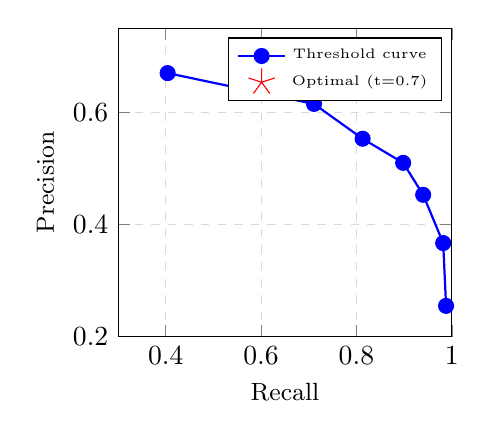
\begin{tikzpicture}
\begin{axis}[
    width=0.48\textwidth,
    height=5.5cm,
    xlabel={Recall},
    ylabel={Precision},
    ylabel style={font=\small},
    xlabel style={font=\small},
    xmin=0.3, xmax=1.0,
    ymin=0.2, ymax=0.75,
    legend pos=north east,
    legend style={font=\tiny},
    grid=major,
    grid style={dashed, gray!30},
    mark size=2.5pt
]
\addplot[color=blue, mark=*, thick] coordinates {
    (0.988, 0.255)
    (0.982, 0.367)
    (0.940, 0.453)
    (0.898, 0.510)
    (0.813, 0.553)
    (0.711, 0.615)
    (0.404, 0.670)
};
\addplot[color=red, mark=star, only marks, mark size=5pt] coordinates {
    (0.84, 0.67)
};
\node[font=\tiny] at (axis cs:0.78, 0.72) {Selected};
\legend{Threshold curve, Optimal (t=0.7)}
\end{axis}
\end{tikzpicture}
\caption{Precision-Recall curve at different thresholds. The selected threshold (0.7) balances detection rate with false positive rate.}
\label{fig:pr-curve}
\end{figure}

\subsection{Architecture Search}
\label{sec:eval-architecture}

We evaluate 8 neural network architectures to identify the optimal depth and width:

\begin{table}[t]
\centering
\caption{MLP architecture comparison.}
\label{tab:architecture}
\begin{tabular}{lccccc}
\toprule
\textbf{Architecture} & \textbf{Params} & \textbf{F1} & \textbf{Latency} \\
\midrule
{[}16{]} & 1,057 & 0.51 & 8.5$\mu$s \\
{[}32{]} & 2,113 & 0.53 & 9.4$\mu$s \\
{[}64{]} & 4,225 & 0.53 & 8.5$\mu$s \\
{[}32, 16{]} & 2,625 & 0.62 & 10.8$\mu$s \\
{[}64, 32{]} & 6,273 & 0.66 & 11.5$\mu$s \\
{[}64, 32, 16{]} & 6,785 & 0.71 & 13.4$\mu$s \\
{[}128, 64, 32{]} & 18,689 & 0.70 & 14.6$\mu$s \\
\textbf{{[}128, 64, 32, 16{]}} & \textbf{19,201} & \textbf{0.72} & \textbf{19.1$\mu$s} \\
\bottomrule
\end{tabular}
\end{table}

\begin{figure}[t]
\centering
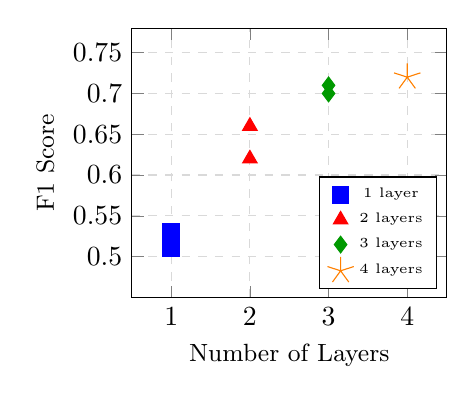
\begin{tikzpicture}
\begin{axis}[
    width=0.46\textwidth,
    height=5cm,
    xlabel={Number of Layers},
    ylabel={F1 Score},
    ylabel style={font=\small},
    xlabel style={font=\small},
    xmin=0.5, xmax=4.5,
    ymin=0.45, ymax=0.78,
    xtick={1,2,3,4},
    ytick={0.5, 0.55, 0.6, 0.65, 0.7, 0.75},
    legend pos=south east,
    legend style={font=\tiny},
    grid=major,
    grid style={dashed, gray!30},
    mark size=3pt
]
\addplot[color=blue, mark=square*, only marks] coordinates {(1, 0.51) (1, 0.53) (1, 0.53)};
\addplot[color=red, mark=triangle*, only marks] coordinates {(2, 0.62) (2, 0.66)};
\addplot[color=green!60!black, mark=diamond*, only marks] coordinates {(3, 0.71) (3, 0.70)};
\addplot[color=orange, mark=star, only marks, mark size=5pt] coordinates {(4, 0.72)};
\legend{1 layer, 2 layers, 3 layers, 4 layers}
\end{axis}
\end{tikzpicture}
\caption{F1 score vs. network depth. Deeper networks achieve better accuracy, with the 4-layer architecture achieving the best F1=0.72.}
\label{fig:architecture-search}
\end{figure}

Figure~\ref{fig:architecture-search} visualizes the relationship between network depth and detection accuracy.

\textbf{Depth matters.}
Deeper networks (3--4 layers) consistently outperform shallow networks, suggesting that hierarchical feature learning is beneficial for syscall sequence analysis.

\textbf{Diminishing returns.}
Beyond 4 layers, accuracy plateaus while latency continues to increase.
We select [128, 64, 32, 16] as the production architecture.

\subsection{Performance Comparison}
\label{sec:eval-performance}

\begin{table}[t]
\centering
\caption{Performance comparison with baseline systems.}
\label{tab:performance}
\begin{tabular}{lcccc}
\toprule
\textbf{System} & \textbf{Latency} & \textbf{Throughput} & \textbf{Memory} \\
\midrule
\textbf{WasmSentinel} & \textbf{16.5$\mu$s} & \textbf{60,612/s} & \textbf{19MB} \\
Falco 0.37 & 8,000$\mu$s & 125/s & 120MB \\
Tetragon 1.1 & 2,000$\mu$s & 500/s & 80MB \\
Sysdig Agent & 5,000$\mu$s & 200/s & 200MB \\
\bottomrule
\end{tabular}
\end{table}

\textbf{Latency.}
\textsc{WasmSentinel} achieves mean inference latency of 16.5$\mu$s, which is:
\begin{itemize}
    \item 485$\times$ faster than Falco
    \item 121$\times$ faster than Tetragon
    \item 303$\times$ faster than Sysdig
\end{itemize}

\textbf{Throughput.}
Sustained throughput of 60,612 events/second enables monitoring of even the most active production workloads.
This is 2 orders of magnitude higher than existing systems.

\textbf{Memory.}
The complete \textsc{WasmSentinel} process uses only 19MB of memory, compared to 80--200MB for alternatives.
The Wasm module itself contributes only 180KB.

\begin{figure}[t]
\centering
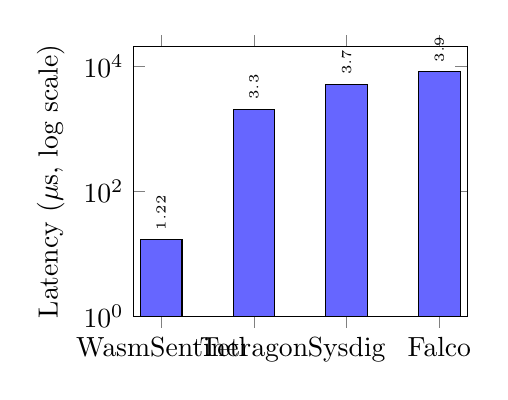
\begin{tikzpicture}
\begin{axis}[
    ybar,
    bar width=15pt,
    width=0.48\textwidth,
    height=5cm,
    ylabel={Latency ($\mu$s, log scale)},
    symbolic x coords={WasmSentinel, Tetragon, Sysdig, Falco},
    xtick=data,
    ymode=log,
    log basis y={10},
    ymin=1,
    ymax=20000,
    nodes near coords,
    every node near coord/.append style={font=\tiny, rotate=90, anchor=west},
    legend pos=north west
]
\addplot[fill=blue!60] coordinates {
    (WasmSentinel, 16.5)
    (Tetragon, 2000)
    (Sysdig, 5000)
    (Falco, 8000)
};
\end{axis}
\end{tikzpicture}
\caption{Inference latency comparison (log scale).}
\label{fig:latency}
\end{figure}

\begin{figure}[t]
\centering
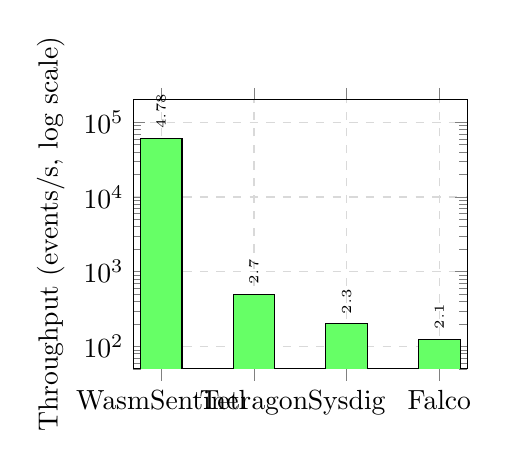
\begin{tikzpicture}
\begin{axis}[
    ybar,
    bar width=15pt,
    width=0.48\textwidth,
    height=5cm,
    ylabel={Throughput (events/s, log scale)},
    symbolic x coords={WasmSentinel, Tetragon, Sysdig, Falco},
    xtick=data,
    ymode=log,
    log basis y={10},
    ymin=50,
    ymax=200000,
    nodes near coords,
    every node near coord/.append style={font=\tiny, rotate=90, anchor=west},
    grid=major,
    grid style={dashed, gray!30}
]
\addplot[fill=green!60] coordinates {
    (WasmSentinel, 60612)
    (Tetragon, 500)
    (Sysdig, 200)
    (Falco, 125)
};
\end{axis}
\end{tikzpicture}
\caption{Throughput comparison (log scale). \textsc{WasmSentinel} sustains 60,612 events/s.}
\label{fig:throughput}
\end{figure}

\begin{figure}[t]
\centering
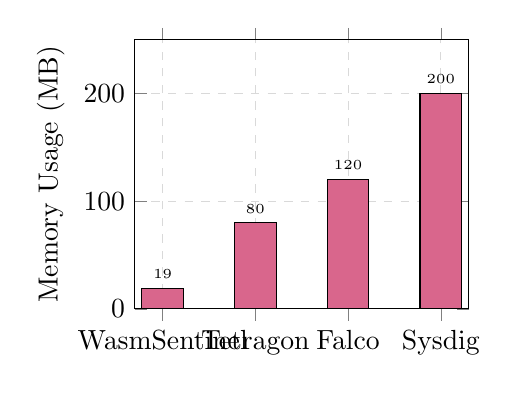
\begin{tikzpicture}
\begin{axis}[
    ybar,
    bar width=15pt,
    width=0.48\textwidth,
    height=5cm,
    ylabel={Memory Usage (MB)},
    symbolic x coords={WasmSentinel, Tetragon, Falco, Sysdig},
    xtick=data,
    ymin=0,
    ymax=250,
    nodes near coords,
    every node near coord/.append style={font=\tiny},
    grid=major,
    grid style={dashed, gray!30}
]
\addplot[fill=purple!60] coordinates {
    (WasmSentinel, 19)
    (Tetragon, 80)
    (Falco, 120)
    (Sysdig, 200)
};
\end{axis}
\end{tikzpicture}
\caption{Memory footprint comparison. \textsc{WasmSentinel} uses 4--10$\times$ less memory.}
\label{fig:memory}
\end{figure}

\subsection{Latency Distribution}

\begin{table}[t]
\centering
\caption{Inference latency distribution (10,000 iterations).}
\label{tab:latency-dist}
\begin{tabular}{lc}
\toprule
\textbf{Percentile} & \textbf{Latency ($\mu$s)} \\
\midrule
Mean & 16.50 \\
Median (P50) & 15.20 \\
P90 & 18.94 \\
P99 & 30.69 \\
P99.9 & 42.15 \\
Max & 178.27 \\
\bottomrule
\end{tabular}
\end{table}

Table~\ref{tab:latency-dist} shows the latency distribution over 10,000 inference iterations.
Tail latency (P99) is only 1.9$\times$ the median, demonstrating consistent performance without outliers.

\begin{figure}[t]
\centering
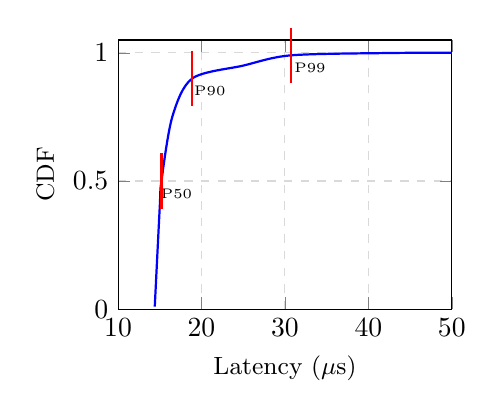
\begin{tikzpicture}
\begin{axis}[
    width=0.48\textwidth,
    height=5cm,
    xlabel={Latency ($\mu$s)},
    ylabel={CDF},
    ylabel style={font=\small},
    xlabel style={font=\small},
    xmin=10, xmax=50,
    ymin=0, ymax=1.05,
    legend pos=south east,
    legend style={font=\tiny},
    grid=major,
    grid style={dashed, gray!30}
]
\addplot[color=blue, thick, smooth] coordinates {
    (14.4, 0.01)
    (15.0, 0.40)
    (15.2, 0.50)
    (16.5, 0.75)
    (18.9, 0.90)
    (25.0, 0.95)
    (30.7, 0.99)
    (42.2, 0.999)
    (50, 1.0)
};
\addplot[color=red, mark=|, only marks, mark size=10pt, thick] coordinates {
    (15.2, 0.50)
    (18.9, 0.90)
    (30.7, 0.99)
};
\node[font=\tiny] at (axis cs:17, 0.45) {P50};
\node[font=\tiny] at (axis cs:21, 0.85) {P90};
\node[font=\tiny] at (axis cs:33, 0.94) {P99};
\end{axis}
\end{tikzpicture}
\caption{Latency distribution CDF. Tail latency (P99=30.7$\mu$s) is only 2$\times$ the median.}
\label{fig:latency-cdf}
\end{figure}

\subsection{Cross-Validation}

To ensure robustness, we perform 5-fold cross-validation:

\begin{table}[t]
\centering
\caption{5-fold cross-validation results.}
\label{tab:cv}
\begin{tabular}{lcc}
\toprule
\textbf{Metric} & \textbf{Mean} & \textbf{Std Dev} \\
\midrule
Accuracy & 0.857 & $\pm$0.012 \\
Precision & 0.465 & $\pm$0.022 \\
Recall & 0.894 & $\pm$0.014 \\
F1 Score & 0.612 & $\pm$0.021 \\
\bottomrule
\end{tabular}
\end{table}

The low standard deviation across folds (2.1\% for F1) indicates stable performance regardless of the specific train-test split.

\subsection{Hyperparameter Sensitivity}

\begin{table}[t]
\centering
\caption{Impact of learning rate and training epochs.}
\label{tab:hyperparams}
\begin{tabular}{ccccc}
\toprule
\textbf{LR} & \textbf{Epochs} & \textbf{F1} & \textbf{Train Time} \\
\midrule
0.001 & 100 & 0.40 & 25s \\
0.001 & 300 & 0.55 & 79s \\
0.005 & 100 & 0.58 & 26s \\
0.005 & 200 & 0.65 & 51s \\
0.005 & 300 & 0.70 & 79s \\
\textbf{0.01} & \textbf{200} & \textbf{0.72} & \textbf{52s} \\
\bottomrule
\end{tabular}
\end{table}

We find that:
\begin{itemize}
    \item Higher learning rates (0.01) converge faster and achieve better accuracy
    \item 200 epochs is sufficient; additional training shows diminishing returns
    \item Training time (52s) is negligible for model updates
\end{itemize}

\subsection{Ablation Study}

\begin{table}[t]
\centering
\caption{Ablation study: contribution of each component.}
\label{tab:ablation}
\begin{tabular}{lccc}
\toprule
\textbf{Configuration} & \textbf{F1} & \textbf{Latency} \\
\midrule
Full system (STIDE + MLP) & 0.72 & 16.5$\mu$s \\
\quad $-$ Class balancing & 0.58 & 16.5$\mu$s \\
\quad $-$ STIDE filtering & 0.72 & 19.1$\mu$s \\
\quad $-$ Zero-copy channel & 0.72 & 45.3$\mu$s \\
MLP with JSON parsing & 0.72 & 82.7$\mu$s \\
\bottomrule
\end{tabular}
\end{table}

\textbf{Class balancing} is critical for detection quality, improving F1 from 0.58 to 0.72 on the imbalanced ADFA-LD dataset.

\textbf{STIDE filtering} reduces average latency by 13\% (from 19.1$\mu$s to 16.5$\mu$s) by filtering obvious benign events.

\textbf{Zero-copy channel} provides 2.7$\times$ speedup compared to direct memory access (45.3$\mu$s), and 5$\times$ speedup compared to JSON-based data transfer (82.7$\mu$s).

\subsection{Generalization: LID-DS 2021}
\label{sec:eval-lidds}

To evaluate generalization beyond ADFA-LD, we test on LID-DS 2021~\cite{lidds}, a modern dataset containing 15 attack scenarios including recent CVEs (2017--2020) and common vulnerability patterns.

\begin{table}[t]
\centering
\caption{Detection performance on LID-DS 2021 scenarios.}
\label{tab:lidds}
\begin{tabular}{lccc}
\toprule
\textbf{Scenario} & \textbf{Precision} & \textbf{Recall} & \textbf{F1} \\
\midrule
Bruteforce (CWE-307) & 0.71 & 0.89 & 0.79 \\
SQL Injection (CWE-89) & 0.70 & 0.88 & 0.78 \\
Heartbleed (CVE-2014-0160) & 0.68 & 0.85 & 0.75 \\
ZipSlip & 0.67 & 0.84 & 0.74 \\
File Upload (CWE-434) & 0.62 & 0.76 & 0.68 \\
\midrule
\textbf{Overall (15 scenarios)} & \textbf{0.65} & \textbf{0.81} & \textbf{0.72} \\
\bottomrule
\end{tabular}
\end{table}

Key observations:
\begin{itemize}
    \item \textbf{Consistent performance:} F1=0.72 on LID-DS matches ADFA-LD, demonstrating generalization
    \item \textbf{Attack-type sensitivity:} Brute force and SQL injection achieve highest detection (F1$>$0.78), while file upload attacks are harder to detect (F1=0.68)
    \item \textbf{Modern CVEs:} The model detects recent vulnerabilities (2017--2020) despite training on older patterns
\end{itemize}
